%
% subsystems.tex
%
% Copyright (C) 2021 by SpaceLab.
%
% FloripaSat-2 Documentation
%
% This work is licensed under the Creative Commons Attribution-ShareAlike 4.0
% International License. To view a copy of this license,
% visit http://creativecommons.org/licenses/by-sa/4.0/.
%

%
% \brief Subsystems chapter.
%
% \author Gabriel Mariano Marcelino <gabriel.mm8@gmail.com>
%
% \institution Universidade Federal de Santa Catarina (UFSC)
%
% \version 0.1.0
%
% \date 2020/06/06
%

\chapter{Subsystems} \label{ch:subsystems}

This chapter presents a description of all subsystems of the space segment of the mission, which can be seen in the exploded view of the satellite, available in \autoref{fig:exploded-view}.

\begin{figure}[!ht]
    \begin{center}
        \includegraphics[width=\textwidth]{figures/exploded-view}
        \caption{Exploded view of the FloripaSat-2 satellite.}
        \label{fig:exploded-view}
    \end{center}
\end{figure}

Most of the subsystems presented here have their own documentation, with a deeper technical description of it. When available, there is a reference to the respective document. This chapter is intended to show an overview of each subsystem, in a macro context of the mission.

\section{On-Board Data Handling}

The OBDH\nomenclature{\textbf{OBDH}}{\textit{On-Board Data Handling}.} 2.0 is an On-Board Computer (OBC) module designed for nanosatellites. The module is responsible for synchronizing actions and the data flow between other modules (i.e., power module, communication module, payloads) and the Earth segment. It packs the generated data into data frames and transmit back to Earth through a communication module, or stores it on a non-volatile memory for later retrieval. Commands sent from Earth segment to the CubeSat are received by radio transceivers located in the communication module and redirected to the OBDH, which takes the appropriate action or forward the commands to the target module.

The module is a direct upgrade from the OBDH of FloripaSat-1 \cite{floripasat}, which grants a flight heritage rating. The improvements focus on providing a cleaner and more generic implementation in comparison with the previous version, more reliability in software and hardware implementations, and adaptations for the new mission requirements. The board of the module can be seen in \autoref{fig:obdh2}.

\begin{figure}[!ht]
    \begin{center}
        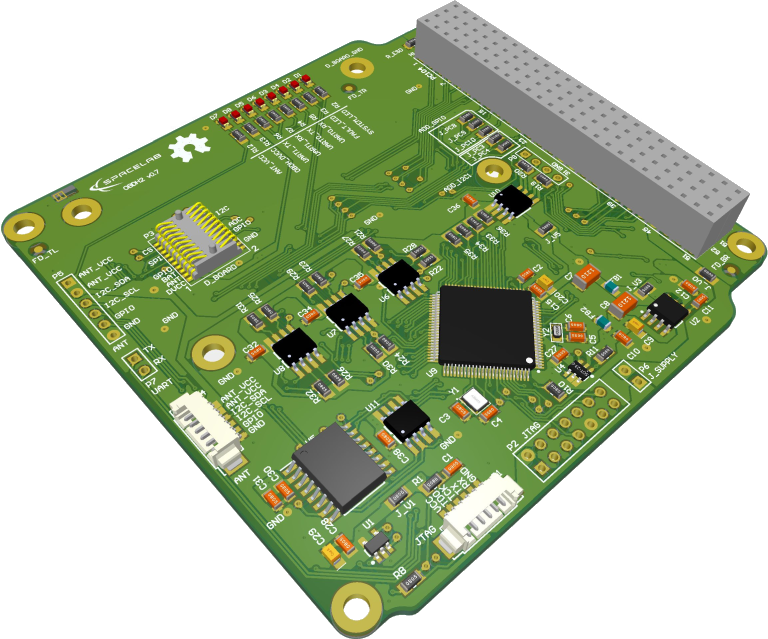
\includegraphics[width=0.7\textwidth]{figures/obdh2-pcb-3d}
        \caption{OBDH module.}
        \label{fig:obdh2}
    \end{center}
\end{figure}

More information about this module can be found in \cite{obdh2}.

\section{Telemetry, Tracking and Command Module}

The TTC\nomenclature{\textbf{TTC}}{\textit{Telemetry, Tracking and Command Module}.} (or TT\&C) is responsible to make the communication between the earth (a ground station) and the satellite, and is divided in two sub-modules: Beacon and downlink/uplink. The beacon is a independent sub-module who transmits a periodic signal containing an identification data (ID) of the satellite and some basic telemetry data. The downlink/uplink sub-module is the main communication device. It has a bidirectional data link to receive telecommands from the earth and transmit all available data back to Earth. The board of the module can be seen in \autoref{fig:ttc}.

\begin{figure}[!ht]
    \begin{center}
        \includegraphics[width=0.7\textwidth]{figures/ttc_board}
        \caption{TTC module.}
        \label{fig:ttc}
    \end{center}
\end{figure}

More information about this module can be found in \cite{ttc}.

\subsection{Antenna Module}

The used antenna module is the CubeSat deployable VHF and UHF antenna from ISISpace \cite{isis-antenna}. It is a four monopole antenna built with tape strings (up to 55 cm) and compliant with the CubeSat standard (dipole or turnstile options are also available). The deployment method is the burning wire and it can be controlled digitally through a I$^{2}$C interface. To allow redundancy, there are two independent deployment controllers that can be activated separately. Also, the construction of this module allows the installation of a solar panel at the top side. The RF gain is about 0 dBi.

A picture of the antenna module (with all antennas released) can be seen in \autoref{fig:isis-antenna}.

\begin{figure}[!ht]
    \begin{center}
        \includegraphics[width=0.8\textwidth]{figures/isis-antenna}
        \caption{Antenna module from ISISpace.}
        \label{fig:isis-antenna}
    \end{center}
\end{figure}

The chosen configuration for this mission can be seen below (using \autoref{fig:isis-antenna-ref} as reference):

\begin{itemize}
    \item Configuration: 4 monopoles (1x VHF + 3x UHF)
        \begin{itemize}
            \item Antenna 1: VHF - 145,97 MHz (beacon)
            \item Antenna 2: UHF - 401,635 MHz (EDC)
            \item Antenna 3: UHF - 436,9 MHz (downlink/uplink)
            \item Antenna 4: UHF - 401,635 MHz (redundant EDC)
        \end{itemize}
    \item Tuning structure size: 2U
    \item Mounting position: Top
    \item Supply voltage: 3,3 V
    \item I$^{2}$C control type: Dual bus
        \begin{itemize}
            \item Primary I$^{2}$C address: 31h (7-bit address)
            \item Redundant I$^{2}$C address: 32h (7-bit address)
        \end{itemize}
    \item I$^{2}$C watchdog: Enabled with a time out of 60 seconds.
\end{itemize}

\begin{figure}[!ht]
    \begin{center}
        \includegraphics[width=0.7\textwidth]{figures/isis-antenna-ref}
        \caption{Configuration reference of the antenna module.}
        \label{fig:isis-antenna-ref}
    \end{center}
\end{figure}

In the digital interface, a temperature sensor and the state of four deployment switches (1 per monopole) are also available. These switches indicate if a monopole is released or not, and can be used as feedback of the deployment process.

\section{Electrical Power System}

The EPS\nomenclature{\textbf{EPS}}{\textit{Electrical Power System}.} is the module designed to harvest, store and distribute energy for the satellite. The energy harvesting system is based on solar energy conversion through te solar panels attached to the CubeSat structure. The EPS is designed to operate the solar panels at their maximum power point (MPPT\nomenclature{\textbf{MPPT}}{\textit{Maximum Power Point Tracking}.}). The board also measures the solar panels current, voltage and the temperature of the batteries. The harvested solar energy is stored in a battery module connected to the EPS. The energy distribution is done by several integrated buck DC-DC converters. The full EPS system is composed of the solar panels, the EPS PCB\nomenclature{\textbf{PCB}}{\textit{Printed Circuit Board.}} and the battery module. A general view of the EPS board can be seen in \autoref{fig:eps2}.

\begin{figure}[!ht]
    \begin{center}
        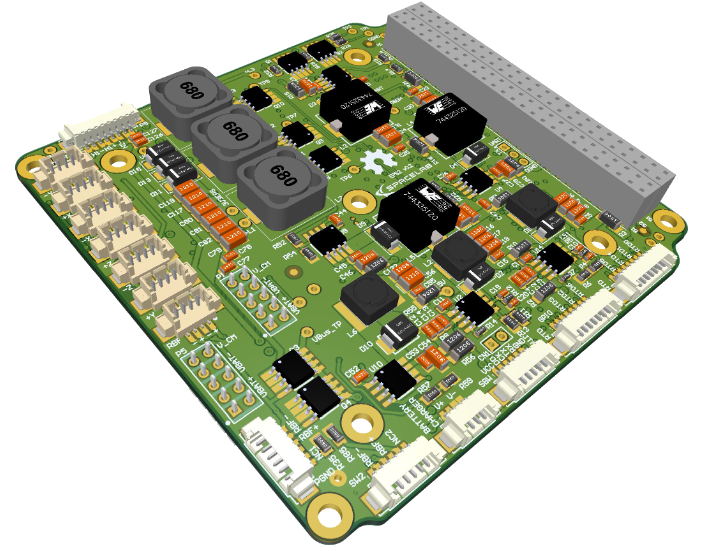
\includegraphics[width=0.7\textwidth]{figures/eps2-pcb-3d}
        \caption{EPS module.}
        \label{fig:eps2}
    \end{center}
\end{figure}

The module is a direct upgrade from the EPS of FloripaSat-1 \cite{floripasat}, which grants a flight heritage rating. The improvements focus on providing a cleaner and more generic implementation in comparison with the previous version, more reliability in software, and adaptations for the new mission requirements.

More information about this module can be found in \cite{eps2}.

\subsection{Battery Module}

The used battery module is the ``\textit{Battery Module 4C}'', that is a separate battery module from the EPS board and composed by four lithium-ion 18650 cells. Besides the cells, the board has connectors for interfacing signals and power lines with the EPS module, 2 power resistors to operate as heaters to maintain the cell's temperature during eclipse periods, and 4 temperature sensors. The batteries used are the ICR18650-30B lithium-ion cells from Samsung \cite{icr18650-30b}, which are connected in series and parallel (two sets of two parallel cells in series) to supply the required voltage and current. Each cell is fixed with 18650 metal holders and between the pairs there is the power resistor attached with a thermal element in the middle. A mechanical mount is placed over the batteries and screwed to the board, providing better stress resistance. Also, there are PC-104 through hole pads present on the board for a connector that could be used for making mechanical integration with the EPS, or with future improvements a interface for power, data or control signals. The board is a direct improvement from the first battery board used in the FloripaSat-1 mission \cite{floripasat}.

\begin{figure}[!ht]
    \begin{center}
        \includegraphics[width=0.7\textwidth]{figures/bat2-pcb-3d}
        \caption{Battery module board.}
        \label{fig:battery-module-board}
    \end{center}
\end{figure}

More information about the battery module can be found in \cite{bat4c}.

\subsection{Solar Panels}

The solar panels are a set of 5 custom made panels manufactured by ORBITAL, a Brazilian company, and a single panel from ISISpace. The panels features protection diodes and high-efficiency solar cells, which are the CESI's CTJ-30 \cite{ctj30} with dimensions 6,9 $\times$ 3,9 cm (area 26,5 cm$^{2}$). This cell is qualified for space use by ESA with an efficiency of 29,5 \% (AM0, BOL). The panels do not include magnetorquers, sensors and others devices. The top solar panel is a model from ISISpace to ensure mechanical compatibility with the antenna module (also from ISISpace). These two types of solar panels can be seen in Figures \ref{fig:solar-panel-orbital} and \ref{fig:top-solar-panel}.

\begin{figure}[!ht]
    \begin{center}
        \includegraphics[width=0.7\textwidth]{figures/orbital-solar-panel}
        \caption{Conceptual solar panel from ORBITAL.}
        \label{fig:solar-panel-orbital}
    \end{center}
\end{figure}

\begin{figure}[!ht]
    \begin{center}
        \includegraphics[width=0.6\textwidth]{figures/isis-top-solar-panel}
        \caption{Top solar panel from ISISpace.}
        \label{fig:top-solar-panel}
    \end{center}
\end{figure}

\subsection{Kill-Switches and RBF}

Two electronic switches have been implemented into the design as to allow for the (redundant) deployment detection of the CubeSat when it is deployed from the POD. This electronic microswitch can be used to prevent the satellite from starting up during launch as is required for all CubeSat launches and hence acts as a Kill-Switch. The Kill-Switch is the Panasonic AV4 microswitch (AV402461), as can be seen in \autoref{fig:av402461}.

\begin{figure}[!ht]
    \begin{center}
        \includegraphics[width=0.25\textwidth]{figures/av402461}
        \caption{Panasonic AV402461 Microswitch.}
        \label{fig:av402461}
    \end{center}
\end{figure}

The Kill-Switch mechanism in the mechanical structure has combined the function of providing deployment and detection (\autoref{fig:kill-switch-installed}). The travel of the actual switch of the Kill-Switch itself is so short that the Kill-Switch could ``detect deployment'' of the CubeSat from the launch adapter simply due to launch vibrations. To overcome this issue the Kill-Switch has been rotated so that there is a positive obstruction in front of the switch which needs 8 mm of deployment before deployment can be detected with the Kill-Switch. In \autoref{fig:kill-switch-installed} the Kill-Switch parts are highlighted and the stowed and deployed configuration is shown.

\begin{figure}[!ht]
    \begin{center}
        \includegraphics[width=0.85\textwidth]{figures/kill-switch-installed}
        \caption{Kill-Switches installed in the mechanical structure.}
        \label{fig:kill-switch-installed}
    \end{center}
\end{figure}

The contact arrangement of the microswitch and the current rating are detailed in \autoref{fig:circuit-kill-switch} and \autoref{tab:kill-switch-specs}.

\begin{figure}[!ht]
    \begin{center}
        \includegraphics[width=0.4\textwidth]{figures/circuit-kill-switch}
        \caption{The contact arrangement of the microswitch.}
        \label{fig:circuit-kill-switch}
    \end{center}
\end{figure}

\begin{table}[!h]
    \centering
    \begin{tabular}{lcccc}
        \toprule[1.5pt]
        \textbf{Characteristic} & \textbf{Minimum} & \textbf{Typical} & \textbf{Maximum} & \textbf{Unit} \\
        \midrule
        Switch Current                      & 2     & 50    & 100   & mA \\
        DC Voltage across switch contacts   & n/a   & n/a   & 30    & V \\
        Contact resistance microswitch      & n/a   & n/a   & 200   & m$\Omega$ \\
        \bottomrule[1.5pt]
    \end{tabular}
    \caption{Kill-Switch current rating and voltage range.}
    \label{tab:kill-switch-specs}
\end{table}

\section{Attitude Control System}

The Attitude Control System (ACS\nomenclature{\textbf{ACS}}{\textit{Attitude Control System}.}) is a passive attitude control system, which depends on the Earth's magnetic field to rotate and stabilize the satellite \cite{santoni2009,gerhardt2010}. The system is composed of one permanent magnet to create a force to align the magnet with the Earth's magnetic field and four hysteresis bars to damp the cube oscillations and achieve stabilization.

When equilibrium is achieved, the permanent magnet aligns itself to the Earth's field lines. The hysteresis bars convert oscillation and rotation energy into heat, maintaining the alignment through magnetic moment. The components are placed in positions as to minimize the magnet's interaction with the hysteresis bars, which limits the magnetic moment of the magnet \cite{francois2010}. \autoref{fig:adcs} shows the mounting of the hysteresis bars (green) and the permanent magnet (red) on the mechanical structure. The whole passive ACS was implemented according to \cite{francois2010}.

\begin{figure}[!ht]
    \begin{center}
        \includegraphics[width=0.7\textwidth]{figures/adcs}
        \caption{ACS subsytem. Rare earth magnet (pink) and hysteresis bars (red) installed in the structure.}
        \label{fig:adcs}
    \end{center}
\end{figure}

As a passive magnetic attitude control system is used, it is possible to stabilize only one axis, and so, the CubeSat will still slowly (due to hysteresis bars) rotate around this axis, even after stabilized. A N45 neodymium magnet and 4 hysteresis bars of Permanorm 5000 H2 are used (courtesy of Vacuumschmelze GmbH \& Co. KG). The material of the hysteresis bar is shaped in order to maximize the stabilization, which is the most important part of the attitude control.

Many conditions impact on the detumbling time, which is the time required for the satellite to stabilize. Magnetic passive attitude stabilization systems such as the one developed for this mission achieve the equilibrium state within a few weeks of operation \cite{santoni2009}.

The FloripaSat-2 satellite does not feature an orbit control subsystem.

\section{Mechanical Structure}

The USIPED 2-Unit CubeSat structure is developed as a generic, modular satellite structure based upon the CubeSat standard. The modular chassis allows for up to two 1-Unit stack of PCBs, or other modules, to be mounted inside the chassis, using the PC-104 standard and spacers attached to the structure. In addition, there are 4 slots in the middle section, providing space for the interface boards and the ACS. The solar panels and antennas are externally mounted, providing a complete mechanical solution. A picture of this structure can be seen in \autoref{fig:usiped-structure}.

\begin{figure}[!ht]
    \begin{center}
        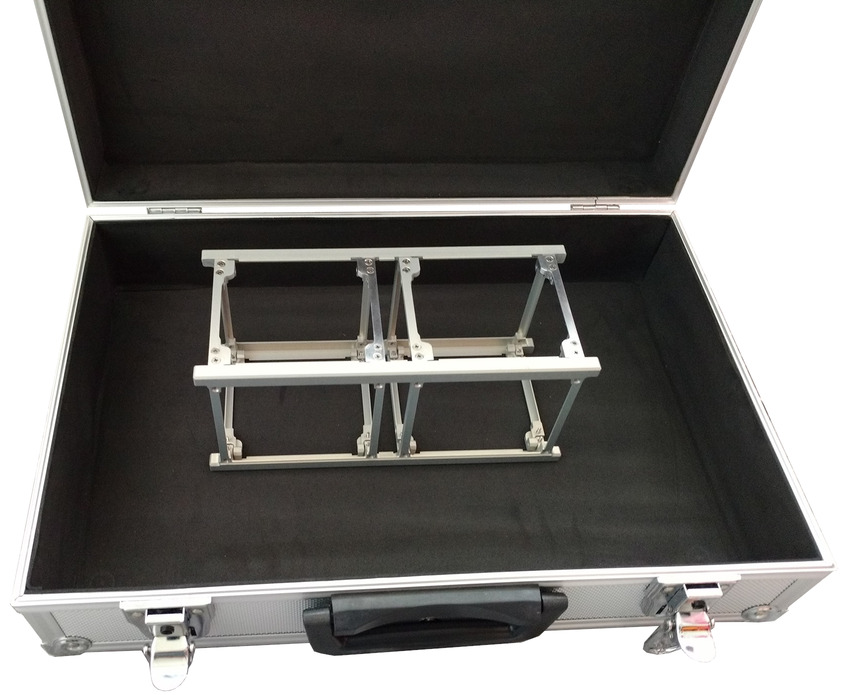
\includegraphics[width=0.7\textwidth]{figures/usiped-2u-structure.jpg}
        \caption{2U CubeSat structure from Usiped.}
        \label{fig:usiped-structure}
    \end{center}
\end{figure}

\section{Interconnection Modules}

\subsection{PC-104 Interconnection Boards}

The PC-104 interconnection boards are intended to be used as an interconnection of the two PC-104 bus segments of the 2U structure (top and bottom units). This interconnection is made with a set of PicoBlade cables between the top and bottom boards. The set of two boards can be seen in \autoref{fig:pc104-adapter}.

\begin{figure}[!ht]
    \begin{center}
        \includegraphics[width=0.7\textwidth]{figures/pc104-adapter}
        \caption{PC-104 adapter boards (top and bottom).}
        \label{fig:pc104-adapter}
    \end{center}
\end{figure}

More information about these boards can be found in \cite{pc104-boards}.

\subsection{External Connection Boards}

The Interstage Interface Panels (IIP) are three vertical internally mounted PCBs designed to give external access up to four modules inside of a 2U CubeSat during final assembly, integration and testing (AIT) before launch. The complete set of the boards allow the nanosatellite to be charged, programed and debugged. The usage of this hardware platform is taking into account the use of a MSP-FET: MSP430 Flash Emulation Tool from Texas Instruments for JTAG programing and debugging, UART debugging through a mini USB type B port interfacing the FT4232H USB bridge IC from FTDI, a JST XH header for charging internal batteries and a Remove Before Flight (RBF) pin header. The boards can seen in \autoref{fig:iip-boards}.

\begin{figure}[!ht]
    \begin{center}
        \includegraphics[width=0.7\textwidth]{figures/iip_fullset}
        \caption{Set of external connection boards.}
        \label{fig:iip-boards}
    \end{center}
\end{figure}

More information about these boards can be found in \cite{iip}.

\section{Payloads}

The FloripaSat-2 satellite is planned to carry three different payloads on-board: ``\textit{EDC}'', ``\textit{Payload-X}'' and the ``\textit{Harsh Payload}''. Each one of these payloads are presented next.

\subsection{Environmental Data Collection}

The Environmental Data Collector (EDC\nomenclature{\textbf{EDC}}{\textit{Environmental Data Collection}.}) is a CubeSat-compatible payload that decodes signals from Platform Transmitter Terminals (PTTs) belonging to the Brazilian Environmental Data Collection System (SBCD\nomenclature{\textbf{SBCD}}{\textit{Sistema Brasileiro de Coleta de Dados}.}) and the Argos-2 System. It is the main payload of the FloripaSat-2 mission.

The main featues of this payload are listed below, a 3D model of the EDC board can be seen in \autoref{fig:edc-board}.

\begin{itemize}
    \item Reception/decoding of SBCD and Argos-2 signals on the 401.635 MHz $\pm$ 30 kHz frequency range.
    \item Can decode up to 12 PTT signals simultaneously.
    \item Attaches a header to decoded messages with frequency, time, and signal strength information.
    \item Full speed I$^{2}$C interface (400 kbit/s) for the OBC communication.
    \item Full-duplex RS-485 interface with fail-safe for the OBC communication.
    \item 5 V power supply.
    \item Memory capable of storing up to 64 decoded user messages.
    \item Generates housekeeping information including current supply, board temperature, digitized signal RMS level, front-end PLL synchronism state and overcurrent events.
    \item Can capture a 2048 samples sequence (16 ms window) from the received signal upon request.
\end{itemize}

\begin{figure}[!ht]
    \begin{center}
        \includegraphics[width=0.6\textwidth]{figures/edc-pcb-top}
        \caption{EDC board.}
        \label{fig:edc-board}
    \end{center}
\end{figure}

As can be seen in \autoref{fig:exploded-view}, for this mission, two identical EDC boards will be used, in a cold redundancy configuration. More information about this payload can be found in \cite{edc}.

\subsection{Redundant OBDH (Payload-X)}

The Payload-X is a radiation-hardened reconfigurable hardware platform designed for a radioactive environment, having as a main feature the possibility to change the hardware configuration of the FPGA\nomenclature{\textbf{FPGA}}{\textit{Field-Programmable Gate Array.}} through remote uplink of its bitstream.

\begin{figure}[!ht]
    \begin{center}
        \includegraphics[width=0.6\textwidth]{figures/payload-x-board}
        \caption{Payload-X board.}
        \label{fig:payload-x-board}
    \end{center}
\end{figure}

More information about this payload can be found in \cite{rigo2019}.

\subsection{Radiation Monitor (Harsh Payload)}

The Radiation Monirot (or Harsh Payload) is a payload capable of evaluate the radiation effects on three SDRAM\nomenclature{\textbf{SDRAM}}{\textit{Synchronous Dynamic Random-Access Memory.}} memories with different manufacturing nodes. This payload will test this chips in the real harsh space environment by flying aboard of FloripaSat-2 CubeSat mission. These particular SDRAM memories were previous characterized on laboratory experiments, then by exposing them to the real environments and executing the same tests routines will not only generate more results for analysis, but also provide an opportunity to assess the test methodologies themselves. Also, after collecting sufficient data to be analysed, this payload could be used to provide a meaningful health status, concerning the radiation doses which the satellite were exposed, to the entire satellite subsystems and further missions. A picture of the harsh payload board is available in \autoref{fig:harsh-payload}.

\begin{figure}[!ht]
    \begin{center}
        \includegraphics[width=0.7\textwidth]{figures/harsh-payload}
        \caption{Radiation monitor board. Top (left) and bottom (right) sides.}
        \label{fig:harsh-payload}
    \end{center}
\end{figure}

In order to accomplish this objectives, the payload is designed to follow the OBDH DaughterBoard standard of SpaceLab, which defines the connectors, shape and size of the board. This standard allows the utilization of the module throughout future SpaceLab core missions in reason of its low space occupation inside the CubeSat, being considered further as an expansion module instead of a payload experiment. A picture of the exploded view of the harsh payload and the OBDH can be seen in \autoref{fig:harsh-payload-integration}.

\begin{figure}[!ht]
    \begin{center}
        \includegraphics[width=0.7\textwidth]{figures/daughterboard-integration}
        \caption{Integration of the radiation monitor payload in the OBDH.}
        \label{fig:harsh-payload-integration}
    \end{center}
\end{figure}

Also, due to the mission limited power budget, the developed board should consider reduce power consumption and define clever power management strategies. In addition, methods for anti latch-up, a type of short circuit which can occur inside an IC, are considered in the design. Therefore, combining all these requirements, the payload architecture consists of the following modules: a control and management subsystem, operated by a System-On-a-Chip (SoC\nomenclature{\textbf{SoC}}{\textit{System-On-a-Chip.}}) solution with an integrated FPGA, power converters for properly voltage level supply, anti latch-up circuitry, communication and interface buses, debug module and the SDRAM memory chips.
